% Page: Linear regression
% sources/stat2004/chapters/inf-06-regression.qmd
% Schematic sample, not a data set from the notes. The line is the least-squares
% fit, which passes through (xbar, ybar). The bands are the page's t intervals
% at confidence 0.95, df = n-2 = 12, t_{12,0.975} = 2.1788.
%   mean:       yhat ± t S sqrt( 1/n + (x-xbar)^2 / Sxx )
%   prediction: yhat ± t S sqrt( 1 + 1/n + (x-xbar)^2 / Sxx )
% S^2 is the unbiased residual variance, divided by n-2.
\documentclass[border=6pt]{standalone}
\usepackage[T1]{fontenc}
\usepackage{lmodern}
\usepackage{amsmath,amssymb}
\usepackage{tikz}
\usepackage{pgfplots}
\usepgfplotslibrary{fillbetween}
\pgfplotsset{compat=1.18}
\definecolor{ink}{HTML}{1F2430}
\definecolor{statblue}{HTML}{174A7E}
\definecolor{bluefill}{HTML}{D7E5F0}
\definecolor{accentfill}{HTML}{F4E4DC}
\definecolor{grey}{HTML}{5E6A75}
\pgfplotsset{
  stat/.style={
    scale only axis,
    axis lines=left,
    axis line style={ink, line width=0.6pt},
    tick style={ink, line width=0.45pt},
    tick label style={font=\small, text=ink},
    label style={font=\small, text=ink},
    title style={font=\small, text=ink, align=center},
    legend style={font=\small, draw=none, fill=none, text=ink,
      cells={anchor=west}, inner sep=1.5pt,
      at={(0.02,0.98)}, anchor=north west},
    unbounded coords=jump,
    scaled ticks=false,
    set layers,
  },
}
\begin{document}
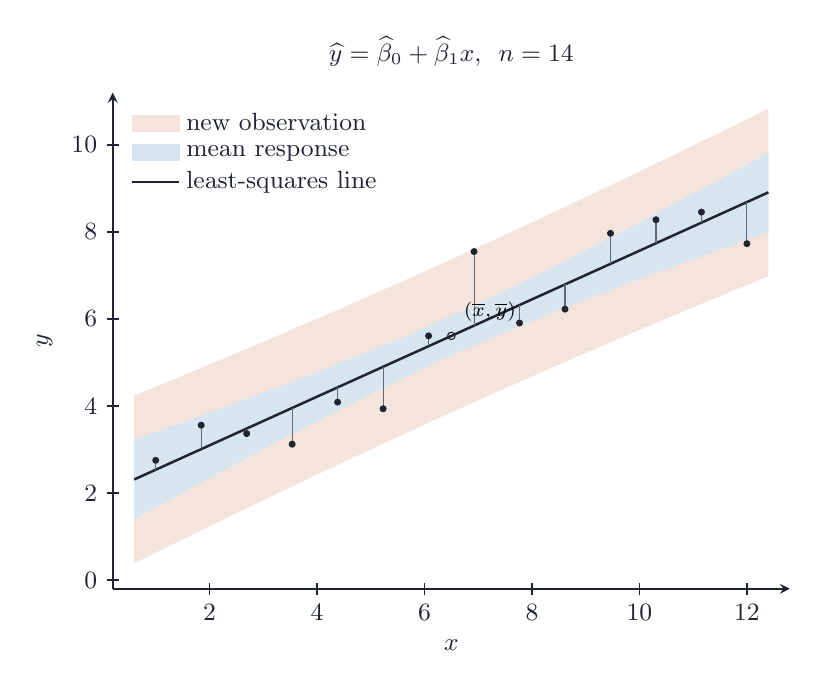
\begin{tikzpicture}
\begin{axis}[
  stat, width=8.6cm, height=6.3cm,
  xmin=0.2, xmax=12.8, ymin=-0.2, ymax=11.2,
  xtick={0,2,4,6,8,10,12},
  ytick={0,2,4,6,8,10},
  xlabel={$x$},
  ylabel={$y$},
  title={$\widehat y=\widehat\beta_0+\widehat\beta_1 x$, \ $n=14$},
  domain=0.6:12.4, samples=61,
]
  \addplot[name path=pu, draw=none, forget plot] {1.976299+0.559119*x + 2.178813*0.780141*sqrt(1+1/14+(x-6.5)^2/162.884615)};
  \addplot[name path=pl, draw=none, forget plot] {1.976299+0.559119*x - 2.178813*0.780141*sqrt(1+1/14+(x-6.5)^2/162.884615)};
  \addplot[accentfill, area legend] fill between[of=pu and pl];
  \addlegendentry{new observation}
  \addplot[name path=mu, draw=none, forget plot] {1.976299+0.559119*x + 2.178813*0.780141*sqrt(1/14+(x-6.5)^2/162.884615)};
  \addplot[name path=ml, draw=none, forget plot] {1.976299+0.559119*x - 2.178813*0.780141*sqrt(1/14+(x-6.5)^2/162.884615)};
  \addplot[bluefill, area legend] fill between[of=mu and ml];
  \addlegendentry{mean response}
  \addplot[ink, line width=0.9pt, samples=2] {1.976299+0.559119*x};
  \addlegendentry{least-squares line}
  \draw[grey, thin] (axis cs:1.0000,2.7514) -- (axis cs:1.0000,2.5354);
  \draw[grey, thin] (axis cs:1.8462,3.5589) -- (axis cs:1.8462,3.0085);
  \draw[grey, thin] (axis cs:2.6923,3.3655) -- (axis cs:2.6923,3.4816);
  \draw[grey, thin] (axis cs:3.5385,3.1220) -- (axis cs:3.5385,3.9547);
  \draw[grey, thin] (axis cs:4.3846,4.0887) -- (axis cs:4.3846,4.4278);
  \draw[grey, thin] (axis cs:5.2308,3.9365) -- (axis cs:5.2308,4.9009);
  \draw[grey, thin] (axis cs:6.0769,5.6115) -- (axis cs:6.0769,5.3740);
  \draw[grey, thin] (axis cs:6.9231,7.5489) -- (axis cs:6.9231,5.8471);
  \draw[grey, thin] (axis cs:7.7692,5.9070) -- (axis cs:7.7692,6.3202);
  \draw[grey, thin] (axis cs:8.6154,6.2249) -- (axis cs:8.6154,6.7933);
  \draw[grey, thin] (axis cs:9.4615,7.9672) -- (axis cs:9.4615,7.2664);
  \draw[grey, thin] (axis cs:10.3077,8.2797) -- (axis cs:10.3077,7.7395);
  \draw[grey, thin] (axis cs:11.1538,8.4558) -- (axis cs:11.1538,8.2126);
  \draw[grey, thin] (axis cs:12.0000,7.7300) -- (axis cs:12.0000,8.6857);
  \addplot[only marks, mark=*, mark size=1.05pt, ink, forget plot] coordinates {
    (1.0000,2.7514) (1.8462,3.5589) (2.6923,3.3655) (3.5385,3.1220)
    (4.3846,4.0887) (5.2308,3.9365) (6.0769,5.6115) (6.9231,7.5489)
    (7.7692,5.9070) (8.6154,6.2249) (9.4615,7.9672) (10.3077,8.2797)
    (11.1538,8.4558) (12.0000,7.7300)
  };
  \draw[ink, thin] (axis cs:6.5,5.6106) circle[radius=1.35pt];
  \node[font=\scriptsize, anchor=south west] at (axis cs:6.55,5.72) {$(\overline x,\overline y)$};
\end{axis}
\end{tikzpicture}
\end{document}
